\documentclass[output=paper]{LSP/langsci} 
\ChapterDOI{10.5281/zenodo.1291932}
\author{Melanie Siegel\affiliation{Hochschule Darmstadt}}
\title{Authoring support for controlled language and machine translation: A report from practice} 
\abstract{Automatic authoring support for controlled language on the one hand and machine translation on the other have previously been seen as two distinct tools in the text processing process. This paper describes methods for the close integration of both, resulting in better written documents as well as machine translation output of higher quality. The methods were implemented in an existing tool for automatic authoring support.}
\maketitle

\begin{document}
\shorttitlerunninghead{Authoring support for controlled language and machine translation}
%melanie.siegel@h-da.de

\section{Introduction}\label{sec:siegel:1}

With the internationalization of the market for technology products and technologies, the demand for translation of technical documentation is increasing. Especially in the European Union there is a raising awareness that it is not sufficient to provide English language documentation, but that documentation needs to be translated into the native language of the users. These translations must be quickly available, upgradable, available in multiple languages simultaneously, and of high quality. At the same time there are significant technological advances in machine translation: there are rule-based and statistical systems, but also hybrid translation methods. More and more companies are supporting their translation efforts with machine translation. Nevertheless, there are several problems:

\begin{itemize}
\item
Users are not familiar with the possibilities and limitations of machine translation. This is why their expectations are not met and they are left disappointed.
\item
To evaluate and test the systems, inappropriate texts, such as prose, are used.
\item
Technical documentation that is translated using machine translation often lacks sufficient quality comparable to texts that are sent to human translators. However, human translators can compensate for this lack of quality in the source document while machine translation systems cannot.
\item
Statistical machine translation systems must be trained on parallel data. Often translation memory data files\footnote{ Translation memory data contains human-translated parallel sentences that professional translators store in a database in order to reuse the translations. For a more detailed description, see \sectref{sec:siegel:3.3}.} are used for training. However, since this data is often accumulated over a number of years and has been originally translated by various different translators, it contains erroneous or inconsistent translations. The machine translation systems trained on this data reflect the heterogeneity of their training data which consequently leads to translations of bad quality.
\end{itemize}

Authoring support with language technology methods aims to support authors in the writing process. Tools based on methods from computational linguistics such as Acrolinx (\url{www.acrolinx.com}) are often used by authors of technical documentation. These tools provide support in checking spelling, grammar, and style, as well as in terminology extraction, terminology checking, and sentence clustering.\footnote{For a detailed description, see \sectref{sec:siegel:3.1}.} Users of authoring support software, on the other hand, make use of translation memory tools, such as \textsc{trados} (\url{www.trados.com}). These tools provide access to previously translated sentences, based on fuzzy matching algorithms. Users of authoring support tools are currently starting to try out machine translation software. Often enough, they are not aware of the possibilities and restrictions of different machine translation methods and tools, which causes them to give up on these tools altogether. For the aforementioned reasons these tools remain distinct, although users already combine them in their daily work.

With the exception of some experiments such as \citet{Roturier2006}, authoring support and machine translation have generally been considered two distinct areas. We want to show that both of these areas can benefit from a combination of methods.

The first goal is to specify some of the possibilities and limitations of machine translation, to deduce options for the authoring of source language documents and to support these through automated processes. 

The second goal is to reduce manual post-editing effort by enhancing the quality of the machine translation output, since experiments (such as \citealt{Allen2001} and \citealt{Plitt2010}) have shown that manual post-editing on high-quality machine translation output is much faster than the process being completed entirely by humans.

We combine methods from machine translation and authoring support and thus enhance the writing as well as the translation process. Methods and processes need to interfere, as authors and translators need to understand the other's way of structuring and processing work. 

To this end we will give an overview of related work that our methods and ideas build upon. We will introduce relevant methods of authoring support, machine translation, and human translation. We will describe how methods from authoring support help users of machine translation to get better performance while explaining at the same time how methods from machine translation can be used in authoring support. 

Experiments and evaluations on which this paper is based have mostly been conducted on German language examples. Rules and methods are implemented using the Acrolinx authoring support software and tested on Google Translate, Langenscheidt T1, and Systran machine translation systems.

\section{Related work}\label{sec:siegel:2}

\citet{BanerjeeEtAl2012} investigate the effect of normalizing source language text, through for example, spell checking, in comparison to data supplementation. They conclude that ``[f]or more noisy datasets [\ldots] normalization does improve translation quality more effectively than data supplementation'' (\citeyear[175]{BanerjeeEtAl2012}). 

\citet{Thurmair2009} lists several pre-editing methods for statistical machine translation: compounding analysis, syntactic pre-processing (well-formed phrases are the only ones that are allowed in the phrase table) and reordering of source language words in a sentence. Our approach to pre-editing is similar to Thurmair's, but focuses on pre-editing rather than on pre-processing, and it tries to find a set of rules that are efficient for pre-editing.

In \citet{Siegel2011} we have shown the impact of controlled language writing on the understandability and translatability of text, as was also done by \citet{Reuther2003}. This research focused on human understanding and translation. Inspired by these ideas, this paper takes a closer look at machine understanding and translation.

\newpage 
\citet{Genzel2010} and others reorder the words in the source language sentence, so that it better fits the word order of the target language. They can show an improvement on the \textsc{bleu} score of the translation. In contrast, we focus on pre-editing mechanisms that tend to have a positive effect on readability, correctness, and consistency of the source language text, as well as on machine translation.

\citet{Hutchins2005} gives examples for controlled English rules that might affect machine translation quality. He does not refer to automatic checking of these rules. 

\citet{Thicke2011} describes the effect of using rules described in the Global English Style Guide \citep{Kohl2008} for pre-editing and terminology adaptations in the machine translation system: ``untrained \textsc{mt} is two times faster to post-edit than to translate from scratch; trained \textsc{mt} is three times faster; and trained \textsc{mt} with source control is four times faster.'' We follow a similar approach to pre-editing, but also include rules that are specific for machine translation, while the Global English Style Guide was assumed for human translation and non-native English.

Various studies, including \citet{OBrien2007} and \citet{AikawaEtAl2007} have shown that pre-editing of the source language text could lead to machine translation quality improvements (in terms of either comprehensibility or post-editing efficiencies). These studies already take automatic rules into account. 

\citet{Plitt2010} evaluate the productivity of using statistical machine translation and post-editing in comparison to human translation. They found that ``the post-editing of statistical machine translation [\ldots] allows translators to substantially increase their productivity'' (\citeyear[15]{Plitt2010}). 
Even more surprising was the result of the quality check: ``To our surprise, translation jobs contained a higher number of mistakes than post-editing jobs'' (\citeyear[14]{Plitt2010}).  
The use of machine translation therefore did not only lead to productivity increase, but also to better translation quality. We go one step further and try to support productivity and translation quality with automatic authoring support in the post-editing process.

\citet{SimardEtAl2007} describe an automatic post-editing method in which a rule-based machine translation system is enhanced with statistical post-editing. This method copes with translation errors concerning terminology. This approach is similar to our idea to use statistical machine translation methods for multilingual terminology extraction and to use the results for terminology checking on the machine translation output in the post-editing phase. However, we propose to leave the post-editing process in the hands of human experts while supporting them with necessary information from the authoring support tool.

\section{Basic methods in authoring support, machine translation, and human translation}\label{sec:siegel:3}

In this section, we describe the methods in authoring support, machine translation, and human translation that are relevant to our approach. Experiments, implementations, and evaluations are based on these methods.

\subsection{Methods in authoring support}\label{sec:siegel:3.1}

Examples for linguistically-based authoring support are Acrolinx (\url{www.acrolinx.com}) and LanguageTool (\url{www.languagetool.org}). These systems first analyse the input using language technology methods, such as tokenization, morphology analysis, and part-of-speech tagging. This linguistic annotation of language data is the basis for further processing steps. We implemented the ideas described in this paper as part of the Acrolinx software and were thus able to build on existing language technology in this tool.

\textsc{Spell checking and grammar checking} can be based on morphology information and rules that detect spelling and grammar errors. Thus, rules that require context information can be implemented, such as in \exref{ex:siegel:1}:

\begin{exe}
\label{ex:siegel:1}
\ex
\begin{xlist}
\ex ``Meine Muttersprache ist Englisch.'' \\
 ``My native language is English.''
\ex ``Das Auto ist englisch.'' \\
``This car is English.''
\end{xlist}
\end{exe}

The words ``Englisch'' and ``englisch'' are written with a capital or a lowercase letter, depending on the context they are used in, and on their syntactic category (\textsc{pos}): it is a noun in the first case and an adjective in the second.

Using the same mechanisms, \textsc{style rules} are defined. Style rules mark language constructions that are not wrong as such, but difficult to understand or not exactly adequate for the respective text type. For example, passive constructions can be hard to understand and should not be used in technical documentation. \citet{Kohl2008} describes style rules for Global English and their implementation in authoring support software.

Closely connected to spell checking is \textsc{terminology checking}. Again, while spell checking marks errors, terminology checking marks words that are not adequate for the text in the domain. The users (who generally work in a group of authors) define a list of terms in a term bank, which are important for the domain and the texts. They also define a list of words that should not be used in that domain. Connecting this user-given information to the general language analysis means that inflectional variants of these terms can be found and marked, such as plural forms. A term variant detection algorithm makes sure that further variants (such as writing a compound with and without a hyphen) are marked as deprecated. In order to set up such a term bank, the user is supported by terminology extraction methods. The aim of terminology extraction is to automatically detect domain terminology in a given corpus. Terminology extraction is carried out using rules that build upon \textsc{pos} information and lemmatization that makes use of morphology information.

The last relevant method is \textsc{sentence clustering}. The authoring support is able to analyze a large amount of text data and find formulation variants, such as ``Stellen Sie die Maschine jetzt an'' and ``Stellen Sie jetzt die Maschine an'' (`turn on the machine'). Here, the word order is distinct but there is no difference in meaning. The user gets the suggestion to always pick one of these variants in order to make the documents more consistent and therefore better translatable.

\subsection{Methods in machine translation}\label{sec:siegel:3.2}

First we look at two basically distinct approaches to machine translation: the statistical approach and the knowledge-based (or rule-based) approach. There are also quite a few attempts to combine the ideas of both, as in \citet{Eisele2009} and in \citet{Thurmair2009}, but a clear distinction at this point makes it easier to evaluate the influence authoring support has on each of the two methods. Some of the processes we propose can contribute to a hybrid machine translation system.

The \textsc{knowledge-based approach} to machine translation makes use of linguistic information and dictionaries to define translation rules based on this information. Examples for such systems are Lucy (www.lucysoftware.com), Langenscheidt T1 (www.langenscheidt.de), and \textsc{systran} (\url{www.systransoft.com}). We expect an effect on the machine translation output when source language texts are more correct and therefore easier to analyze with language rules.

The \textsc{statistical approach} to machine translation analyzes large amounts of parallel data, sets up phrase tables in the source and in the target language and combines the phrases in the translation task. This kind of parallel data is, for example, available in translation memories. Examples for this approach are Google Translate (translate.google.de) and Moses \citep{KoehnEtAl2007}. We expect an effect on the machine translation output when source texts are standardized, giving less variation in formulations of text and training data.

\subsection{Methods in human translation}\label{sec:siegel:3.3}

Most technical translations are carried out with the help of translation memories. \textsc{Translation memories} are databases of sentences that have been professionally translated in previous work. While translating, the translator uses the translation memory database that tries to find sentences similar to the one he or she is about to translate. If a similar sentence is found in the database, it can be re-used in the new translation. \citet{Somers2004} show that the technology of translation memories is similar to example-based translation -- a method that is essential for statistical machine translation which is in widespread use today. This is why it can be said that many translators already use machine translation technology today when using translation memories without realizing that they do. 

The databases that gradually develop from the work of translators are a valuable data source for statistical machine translation. They provide parallel sentences, translated by professional translators. 

\section{Authoring support for better machine translation results}\label{sec:siegel:4}

The language analysis technologies of intelligent authoring support tools provide a basis for improving machine translation: automatic authoring support takes over the tasks of tokenization, \textsc{pos}-tagging, morphology analysis, decomposition, and shallow grammar analysis.

Authoring support provides rules concerning monolingual texts. In the process of translation these rules can be applied to the source language text (pre-editing) and to the target language text (post-editing). Further, authoring support rules and methods can help in the evaluation of machine translation results.

\subsection{Pre-editing: Optimization of source language documents}\label{sec:siegel:4.1}
\largerpage
Often enough, users test machine translation engines using texts that are not suited for that task. Sometimes they run tests with prose texts, such as excerpts from historical literature. Prose typically contains a lot of metaphorical language that is difficult to translate even for human translators. Sometimes they process texts of low quality, full of errors.

Using authoring support in the pre-editing process means to correct spelling and grammar errors in the source document. This example of a translation (of an instructive text) using Langenscheidt T1 demonstrates the effect on data cleaning, as in \exref{ex:siegel:2}:


\begin{exe}
\label{ex:siegel:2}
\ex
\begin{xlist}
\ex
``Achten Sie darauf das der \textsc{lnb} fest am Arm des Spiegels montiert ist.'' \\ ``You pay attention to that that the \textsc{lnb} firmly at the arm of the mirror is mounted.'' 
\ex
``Achten Sie darauf, dass der \textsc{lnb} fest am Arm des Spiegels montiert ist.'' \\ ``Pay attention to the \textsc{lnb} being firmly mounted at the arm of the mirror.''
\end{xlist}
\end{exe}

Consistent and precise terminology helps the machine translation process. If a terminology database is available, checking for terminological consistency supports the machine translation process. For example, in our experiments, the imprecise term ``Kerzenschlüssel'' was translated to ``candle key'' while the precise term ``Zündkerzenschlüssel'' was correctly translated to ``sparking-plug wrench''. Authoring support provides not only methods for terminology checking, but also methods for terminology extraction in order to set up a terminology database, as described in \secref{sec:siegel:3.1}. Terminology extraction rules in software like Acrolinx are based on linguistic information and run on data in the relevant domain. Thus, the extracted terms are more useful than, for example, a general domain-independent ontology.

Authoring support also contains style rules. These are defined along the lines of consistency, clarity, understandability, and translatability of text. Many of these rules are also useful for machine translation pre-editing. Here is an example of a complex sentence structure where the general authoring rule for reformulation is also helpful for machine translation, as in \exref{ex:siegel:3}:

\begin{exe}
\label{ex:siegel:3}
\ex
\begin{xlist} 
\ex ``Eine zu lose Zündkerze hat Wärmestau und schlechte Abdichtung zur Folge, ein zu kräftiges Anziehen hingegen kann das Kerzengewinde und sogar den Zylinderkopf beschädigen.'' \\ ``A too loose spark plug has been able to damage accumulation of heat and bad seal for the consequence a too strong pickup on the other hand the candle thread and even the cylinder head.''
\ex ``Eine zu lockere Zündkerze führt zu Wärmestau und schlechter Abdichtung. Eine zu fest angezogene Zündkerze  kann das Gewinde und den Zylinderkopf beschädigen.'' \\ ``A too loose spark plug leads to accumulation of heat and bad seal. A too firmly absorbed spark plug can damage the thread and the cylinder head.''
\end{xlist} 
\end{exe}

\newpage 
Another area of authoring support that can be of help in machine translation is sentence normalization. Given a large amount of text data in the domain, sentence clustering can find similar sentences and help standardize them. \exref{ex:siegel:4} shows an English sentence cluster found in technical documentation:

\begin{exe}
\label{ex:siegel:4}
\ex
\begin{xlist}
\ex
For more information, consult our web page.
\ex
For more information, consult the web page.
\ex
Go to our web page to find more info.
\end{xlist}
\end{exe}

Authoring support can make sure that in contexts like this only one specific variant is used. If the variant selection is trained on machine translation training data, it can be ensured that in case of variants in the source language text these are changed to 100\% matches in the machine translation training data.

These methods of pre-editing can, on the one hand, be applied by authors, as is usually done in the technical documentation authoring process. Errors are marked so that the author can come up with reformulations. Further, the author gets a better understanding of the abilities and limits of machine translation as such.

On the other hand, it is possible to automatically apply many of these reformulations. In contrast to authoring support of technical documents, the main focus here is on better machine translation results. Automatic application of rules is much faster. It can be the case, however, that the writing style used in the source language text will deteriorate when automatically applying rules without any human intervention whatsoever.

\subsection{Post-editing: Optimization of machine translation output}\label{sec:siegel:4.2}

The authoring support tool works on and processes monolingual text. Therefore, using the same mechanisms as in pre-editing, we can correct spelling, grammar and style errors on the target language text. In order to collect errors to correct in automatic post-editing, we conducted experiments with professional translators performing post-editing on machine translation output. On top of spelling and grammar corrections, we identified rules for automatic post-editing of German machine translation output on this basis. Here are examples of these rules:

\begin{itemize}
\item
correct terminology
\item
correct standard expressions
\item
correct word order
\item
convert future tense to present tense
\item
convert indicative to causative
\item
convert ``man'' to passive
\item
convert series of ``von''+ noun
\end{itemize}

Terminology correction is a major part of the corrected errors and thus requires a specific focus. \citet{Allen2001} shows tools that support humans in manually adding unknown words to a dictionary and in domain-adaptation by manually selecting the best translations of words in a certain domain. We propose to do multilingual term extraction (a method that is part of authoring support), and make use of term bank organization (with domains and linked terms) for the organization of the domain-dependent selection of translations. The terminology can be adapted to the domain by extraction methods working on the training data; a term bank is set up with information about the domain and used for terminology checking on the source and target language texts.

\subsection{Evaluation of machine translation}\label{sec:siegel:4.3}

The authoring tool can also be used to evaluate machine translation results. Already in the project Verbmobil \citep{Wahlster2000} the idea came up to run different machine translation machines in parallel and to choose the best result. What result can be seen as best is dependent on the translation task. In the Verbmobil environment, picking the best result was often enough guided by time restriction because this was a spoken dialogue translation situation, where processing time is crucial. In translating technical documentation, a few seconds more or less are not that important. More important, however, is the actual quality of the machine translation result. The quality can be determined using authoring support along the areas of spelling, grammar, style, and terminology checking of the target language text. Checking results are combined in an evaluation value that can directly be used to choose the best translation.

\section{Machine translation methods for better authoring support}\label{sec:siegel:5}

The benefit of combining authoring support and machine translation is bidirectional because authoring support can also benefit from methods developed for machine translation. The first connection is very basic: some of the rules developed in authoring support for machine translation pre-editing can also be used in authoring support of technical documentation writing. Technical documentation often enough has to be translated to other languages. If the source language document is organized such that it is easier to translate for machine translation systems, it is also easier to translate (and to understand) for humans. Consider the rules concerning reduction of ambiguity, for example. One of these rules requires avoiding anaphoric pronouns. \textsc{mt} translates single sentences and is mostly unable to take care of anaphora resolution. Human translators use translation memories that also consist of single sentences. Therefore, this rule is useful for both.

Another area is the set-up of a term bank for terminology checking. Using paradigms from statistical machine translation, we extract phrase tables from multilingual data. These phrase tables create a foundation to linking both terms between languages, and terms within a particular language.  
The result is that we have within each language synonyms of the extracted terms because these terms were translated in the same way. For example, in German -- English parallel data we found this cluster of words for English because all of these were translated to the German word ``Grundstellung'': starting position, basic position, home position, basic setting, initial position, starting pos., normal position. This word cluster actually builds a synonym cluster. These synonyms can be imported into the term bank and then linked. This information can be used in terminology checking, but also in sentence clustering as a similarity measure.

Finally, the multilingual term extraction results (with statistical machine translation methods) can again be used for rule-based machine translation to enhance the domain-specific dictionaries and for statistical machine translation to make the training data more consistent.

\section{Experiments and evaluations}\label{sec:siegel:6}

\subsection{First experiment: Evaluate what type of authoring support is useful for MT}\label{sec:siegel:6.1}

The goal of the first set of experiments we conducted was to find out how to set up the authoring support system in order to get the best results on machine translation output. We started with only three documents and one rule-based machine translation system, Langenscheidt T1. We applied several existing rules of authoring support and inspected the machine translation behavior. Here spelling and grammar correction on the source text turned out to be an important factor. Further, we found out that rules concerning lexical items, such as the avoidance of ambiguous words, have an important impact on the quality of machine translation. 

\begin{table}
\resizebox{\textwidth}{!}{
\begin{tabular}{lcccr} 
\lsptoprule
& \multicolumn{2}{c}{Google Translate} & \multicolumn{2}{c}{\textsc{systran}}\\
\cmidrule(lr){2-3}\cmidrule(lr){4-5}
{} & English & Italian & English & Italian\\\midrule
Avoiding \textit{man} & 3 & 3 & nn & nn\\
Separation of verb components & 2 &  2 &  2 & 1\\
Fillers &  1 & 1 &  3 & 3\\
Prepositions & 1 & 1 &  nn & nn\\
Word order & 3 & 3 &  nn & nn\\
\textit{can} & 3 & 3 & nn & nn\\
Simple list &  nn & nn &  nn & nn\\
Enumerations  & 3 &  2 &  2 & 2\\
One relative clause  &  3 & 3 &  3 & 3\\
Two relative clauses  & 3 & 3 &  2 & 2\\
Passive  &  3 &  3 &  3 & 2\\
Conditional clauses  &  2 &  2 &  2 & 2\\
Prepositional phrases & 2 &  1 & 2 & 1\\
Questions &  2 &  1 &  1 & 1 \\
Swapping subject-object arguments &  nn &   nn &  3 & 3\\
\lspbottomrule
\end{tabular}
}
\textmd{3: strong improvement, 2: slight improvement, 1: no improvement, nn: improvement not necessary}
\caption{Application of rules and the effect on Google Translate and \textsc{systran} for German--English and German--Italian translation. Adapted from \citet[43]{Klausner2011}.}
\label{tab:siegel:1}
\end{table}

\subsection{Second experiment: Different MT systems and target languages}\label{sec:siegel:6.2}

The next step was to take into account a statistical machine translation system (Google Translate) and a rule-based system (\textsc{systran}) in order to find out if pre-editing rules have more influence on one or the other. Furthermore, we compared the translations German -- English and German -- Italian in order to investigate whether source language correction methods should be dependent on the target language. For the results of this experiment, see \tabref{tab:siegel:1}. We identified style rules that have a similar effect on both machine translation systems. These include, for example, `do not place two parts of a verb too far away from each other in the sentence' (``separation of verb components''), or rules that have a bigger impact on the statistical system, such as `avoid the impersonal pronoun \textit{man'} as well as rules that have an influence on the rule-based-system, such as `use standard word order'. Simple lists can be handled by both machines and both target languages and need not to be converted, while enumerations seem to be a problem in \textsc{mt}.

In this experiment,\footnote{The experiment was supported by Katharina Klausner. For further information see \citet{Klausner2011}.} we could not find any differences in the influence of authoring support rules on machine translation results that can be explained by the structure of English or Italian as a target language. However, the results of the experiment could be used to produce a linguistic resource for authoring support checking, i.e., the 52 style rules 
%\reference
{used in} the following experiments. 

\begin{table}
\resizebox{\textwidth}{!}{
\begin{tabular}{lrrrrd{2}}   
\lsptoprule
& \multicolumn{1}{c}{Evaluation} & Evaluation  I& Evaluation II & Evaluation  III & \multicolumn{1}{c}{Average}     \\
& \multicolumn{1}{c}{(original} & (pre-edited) & (pre-edited) & (pre-edited) &  \multicolumn{1}{c}{evaluations} \\
& \multicolumn{1}{c}{text)} & & &  & \multicolumn{1}{c}{(pre-edited)} \\
\midrule
content words wrong &  42 & 81 & 77 & 37 & 65\\
incorrect punctuation &  11 &  4 &  8 &  4 &  5.33\\
incorrect word forms & 17 &  27 & 7 & 3 & 12.33\\
incorrect word order & 32 & 50 & 30 & 42 & 40.67\\
missing content words &  16 &  1 & 17 &  3 &  7\\
other error & 27\footnote{15.79\%} &  15 &  27 &  19 & 20.33\footnote{11.15\%} \\
wrong functional words &  26 & 34 & 40 & 21 & 31.67\\
\textsc{total} & 171 &  212 &  206 & 129 &  182.33\\
\lspbottomrule
\end{tabular}
}
\caption{Classification of errors in \textsc{mt} output of original text compared to text, where pre-editing rules are applied}
\label{tab:siegel:2}
\end{table}

\subsection{Third experiment: Evaluate the effect of implemented rules on MT results}\label{sec:siegel:6.3}

The aim of the next round of experiments was to evaluate the effect of these rules on machine translation results. To this end, a German text from the Open Office documentation (\url{http://opus.lingfil.uu.se/OpenOffice3.php}) was corrected along the lines of the authoring support checking results. Original and corrected text (about 100 sentences each) were translated using Lucy (rule-based), Moses, and Google Translate (both statistically-based) and their results were classified by translators according to the identified translation errors. 

The error classification (see \tabref{tab:siegel:2}) showed that the translation of the pre-processed text contained more errors that could be classified by professional technical translators. The category ``other error'' contained 15.79\% for the machine translation without pre-editing and only 11.15\% for the machine translation with pre-editing.\footnote{ Other errors could be very different, such as untranslated words as in ``By clicking of this symbol you add a hyperlink of the current \textsc{url} to your document ein.'' or translation close to the (German) source text, such as ``Did you split the page into columns or the cursor is in a multi-column text frame, \ldots''.} It could also be shown that the results contained fewer grammar errors (punctuation, word forms) if pre-editing was performed with the authoring support rules. 

\tabref{tab:siegel:3} shows that there were no machine translation results categorized as correct translations for the non-pre-edited texts, while with pre-edited machine translation, 20\% of the translations were correct. 

\begin{table}
\resizebox{\textwidth}{!}{
\begin{tabular}{lrrrre}   
\lsptoprule
& \multicolumn{1}{c}{Evaluation} & Evaluation  I& Evaluation II & Evaluation  III & \multicolumn{1}{c}{Average}     \\
& \multicolumn{1}{c}{(original} & (pre-edited) & (pre-edited) & (pre-edited) &  \multicolumn{1}{c}{evaluations} \\
& \multicolumn{1}{c}{text)} & & &  & \multicolumn{1}{c}{(pre-edited)} \\
\midrule
1.1. Lucy &  0 &  1\% & 5\% & 10\% &  5.33   \rlap{$\%$}\\
1.2. Moses & 0 &  1\% &   3\% &   9\% &   4.33\rlap{$\%$}\\
Google Translate &  0 &   4\%  & 7\% &  7\% & 6\rlap{$\%$}\\
\textsc{total} &   0 &   7\% & 20\% & 33\% &   20\rlap{$\%$}\\
\lspbottomrule
\end{tabular}
}
\caption{Comparison of sentences classified as correct translations, original and pre-edited sentences}
\label{tab:siegel:3}
\end{table}

\subsection{Fourth experiment: Human post-editing of MT results}\label{sec:siegel:6.4}

In another task (see \tabref{tab:siegel:4}), translators were asked to post-edit machine translation results. We calculated the total word-level Levenshtein distances between machine translation output and post-edited machine translation output. Pre-ed\-iting using authoring support before machine translation processing lead to the reduction of distance (15.82\%) which indicates that post-editing is much less effort when pre-editing was involved as well.

\begin{table}
\begin{tabular}{lr}
\lsptoprule
(Original) & 2225\\
\midrule
I (pre-edited) &  2113\\
II (pre-edited) &   1924\\
III (pre-edited) &  1582\\
average pre-edited &  1873\\
\lspbottomrule
\end{tabular}
\caption{Total word-level Levenshtein distances between machine translation output and post-edited machine translation output}
\label{tab:siegel:4}
\end{table}

\subsection{Fifth experiment: Automatic evaluation of rule impact}\label{sec:siegel:6.5}

In \citet{RoturierEtAl2012}, we introduced a framework to analyze the impact of source re-formulations on machine translation quality using automatic metrics (see \figref{fig:siegel:1}). This approach will enable us to automatically evaluate the effect of pre-editing rules on machine translation quality and therefore to get evaluations on more data. First results show that grammar reformulations (leading to correct grammar) seem to have a large influence on translation quality. 

\begin{figure}
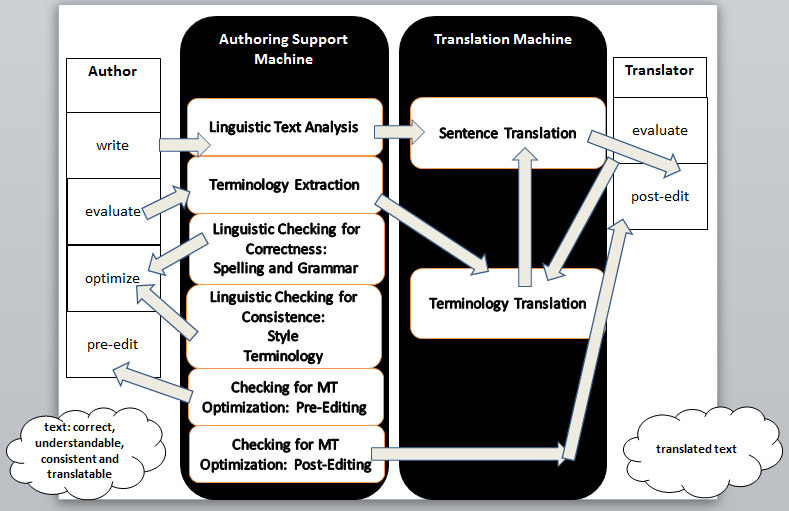
\includegraphics[width=\textwidth]{figures/SiegelF1Crop.png}
\caption{Workflow and Interdependencies in a Combined System}
\label{fig:siegel:1}
\end{figure}  

\section{Summary}\label{sec:siegel:7}

We have shown that methods from automatic authoring support and machine translation can be applied to both tasks. Thus, authoring support and machine translation should be integrated modules in the text production and translation process. Automatic authoring support is monolingual; checking rules can only be applied to either the source language text or the target language text, without taking the translation into account. Therefore, multilingual terminology extraction on \textsc{smt} training data is a first step towards multilingual checking.

In order to further expand the integration, it is necessary to involve more languages in the evaluation tasks. We plan to include Chinese in our inspections. As for the process itself, we will automate the pre- and post-editing process as much as possible and evaluate whether the machine translation results can be optimized with minimal or without any human intervention.

\section*{Acknowledgments}\label{sec:siegel:8}

Most of the work described in this article was carried out when I was part of the company Acrolinx GmbH. We participated in a research project called taraXÜ, financed by TSB Technologiestiftung Berlin -- Zukunftsfonds Berlin, co-financed by the European Union -- European fund for regional development.

\sloppy
\printbibliography[heading=subbibliography,notkeyword=this]

\end{document}
